\chapter{Results}
In this chapter we present the outcome of using CNN's for recovering images from compressed measurements. First, we present the alpha network and its performance using both learning approaches: supervised and unsupervised. We present the training, test and validation error for the dataset \cite{LFWTech}. Afterwards, we also show the images from the test dataset and compare them against the ground truth in terms of PSNR and SSIM. The same data can expected for the beta network. Finally, we present the time measurement that our approach needs for fully reconstructing an image.  

\section{Alpha network supervised training}
The alpha network was describe in section \ref{ch:alphaNet}. It is smaller than the beta network and in the following we show its performance.
\subsection{Supervised training}
For supervised learning we train the network using compressed measurements generated with the matrix $\Phi$. Figure \ref{fig:alphaSupValidPSNR} shows the training of the network for 200 epochs. The blue line is the loss function MSE. The red solid line represents the PSNR on the whole training dataset whereas the red doted line represents the PSNR of the validation dataset. As it can been seen the error on the validation set is not as high as the training error but it is close to what is consider optimum to prevent overfitting. Figure \ref{fig:alphaSupTestPSNR} is the progress on the test dataset over each epoch. Even though the difference is higher, approximately 4 dB, the reconstruction is considerably good. Figures \ref{fig:alphaSupValidSSIM} and \ref{fig:alphaSupTestSSIM} show the progress of SSIM during training. 
 
\begin{figure}[tb] 
\centering 
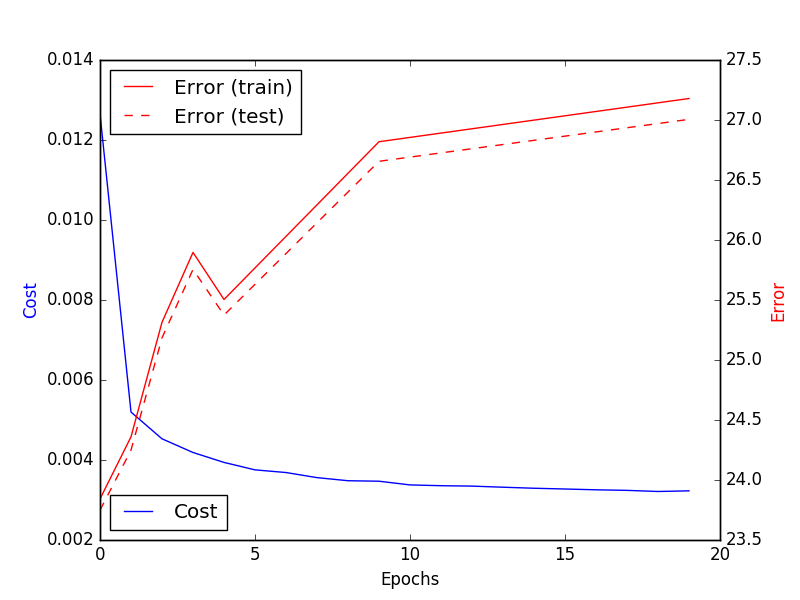
\includegraphics[scale=0.6]{alphaSup_PSNR_VALID_SET.png}
\caption[PSNR validation progress during training of supervised alpha network]{PSNR progress over each epoch of supervised alpha network on validation dataset.}
\label{fig:alphaSupValidPSNR} 
\end{figure}  

\begin{figure}[tb] 
\centering 
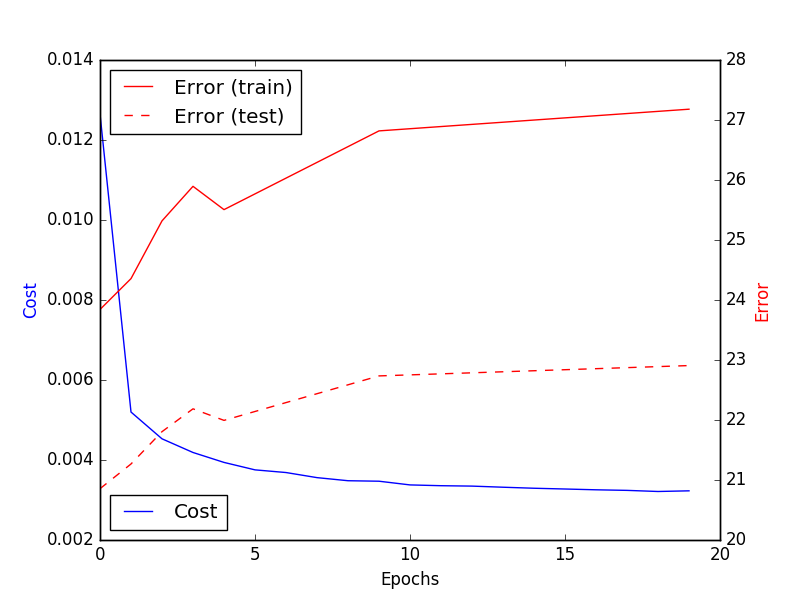
\includegraphics[scale=0.6]{alphaSup_PSNR_TEST_SET.png} 
\caption[PSNR testing progress during training of supervised alpha network]{PSNR progress over each epoch of supervised alpha network on testing dataset.}
\label{fig:alphaSupTestPSNR} 
\end{figure}  

\begin{figure}[tb] 
\centering 
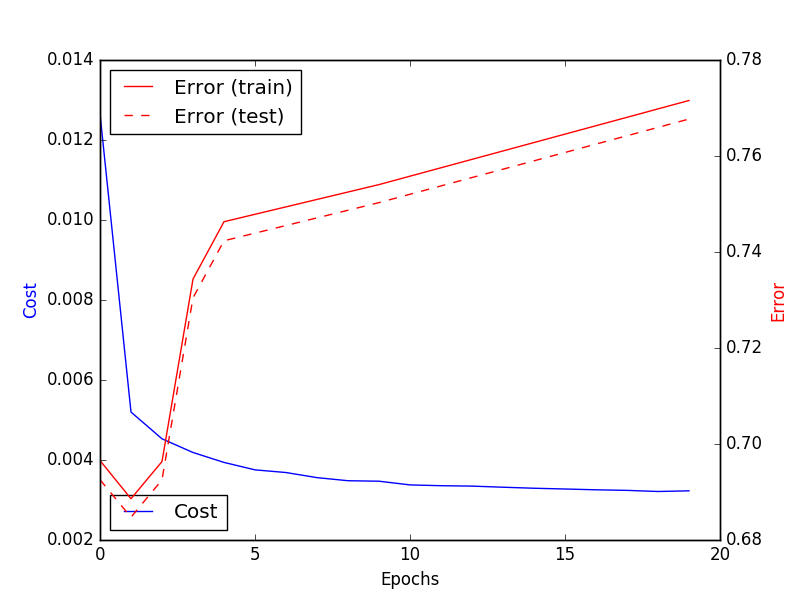
\includegraphics[scale=0.6]{alphaSup_SSIM_VALID_SET.png} 
\caption[SSIM validation progress during training of supervised alpha network]{SSIM progress over each epoch of supervised alpha network on validation dataset.}
\label{fig:alphaSupValidSSIM} 
\end{figure}  

\begin{figure}[tb] 
\centering 
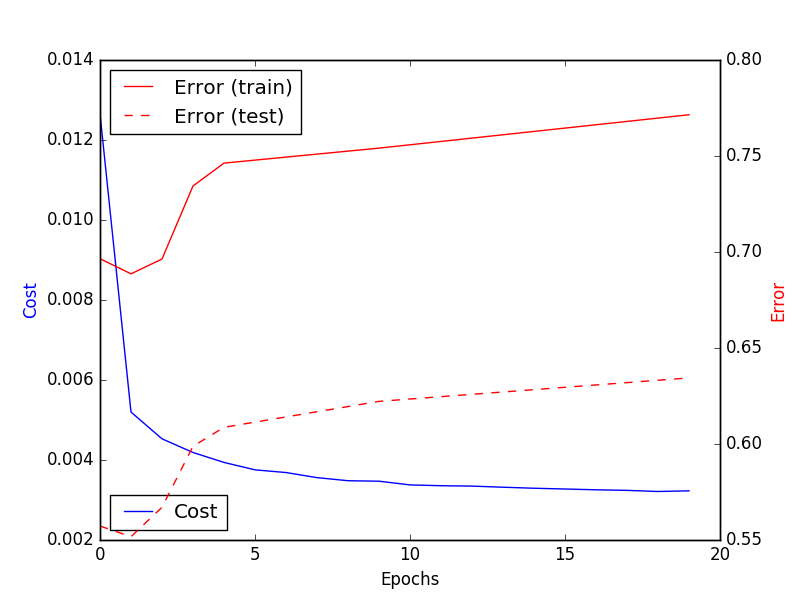
\includegraphics[scale=0.6]{alphaSup_SSIM_TEST_SET.png} 
\caption[SSIM testing progress during training of supervised alpha network]{SSIM progress over each epoch of supervised alpha network on testing dataset.}
\label{fig:alphaSupTestSSIM} 
\end{figure}  

%The reconstructed images from testing dataset using the supervised alpha network are shown in %figure \ref{fig:allReconAlphaSup}.

%\begin{figure}[tb] 
%\centering 
%\includegraphics[scale=1]{alphaSup_ReconAll.png} 
%\caption[Reconstructed testing images with supervised alpha network]{Ground truth, PSNR and %SSIM of reconstructed images from testing dataset using supervised alpha network.}
%\label{fig:allReconAlphaUnsup} 
%\end{figure}  

\FloatBarrier

\subsection{Unsupervised training}
For unsupervised learning the training data was not compressed beforehand. That is, the matrix $\Phi$ is intrinsically learned as the first layer pf the network amd the subsequent layer aim to reconstruct the image. Figures \ref{fig:alphaUnsupValidPSNR} and \ref{fig:alphaUnsupTestPSNR} show the progress of PSNR over 200 epochs on validation and testing sets. Figures \ref{fig:alphaUnsupValidSSIM} and \ref{fig:alphaUnsupTestSSIM}. As it was expected learning the matrix $\Phi$ yielded better results. Namely, there was an increase of approximately 1.2 dB for PSNR and 0.02 for SSIM.    

\begin{figure}[tb] 
\centering 
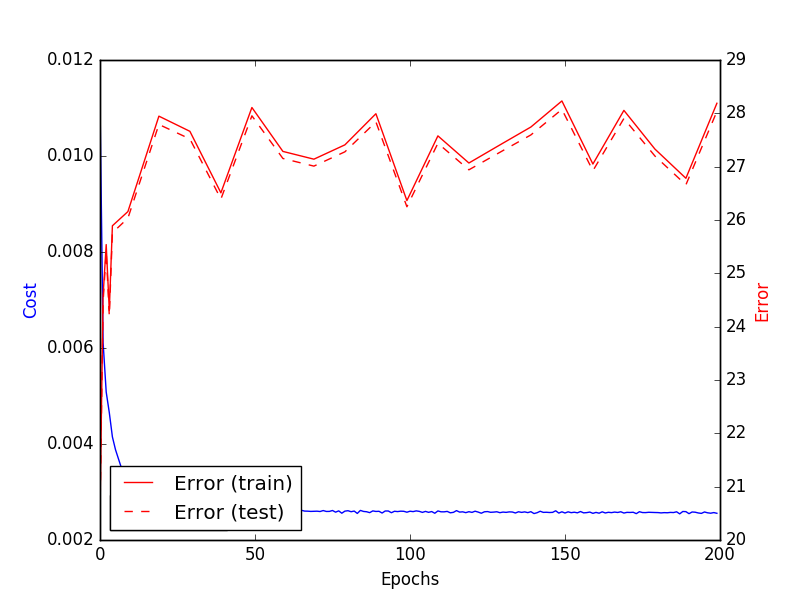
\includegraphics[scale=0.6]{alphaUnsup_PSNR_VALID_SET.png} 
\caption[PSNR validation progress during training of unsupervised alpha network]{PSNR progress over each epoch of unsupervised alpha network on validation dataset.}
\label{fig:alphaUnsupValidPSNR} 
\end{figure}  

\begin{figure}[tb] 
\centering 
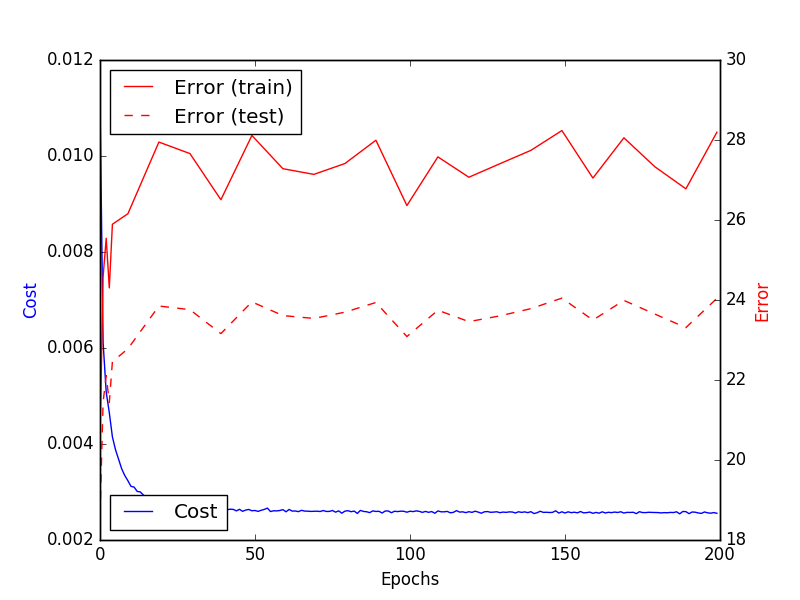
\includegraphics[scale=0.6]{alphaUnsup_PSNR_TEST_SET.png} 
\caption[PSNR testing progress during training of unsupervised alpha network]{PSNR progress over each epoch of unsupervised alpha network on testing dataset.}
\label{fig:alphaUnsupTestPSNR} 
\end{figure}  

\begin{figure}[tb] 
\centering 
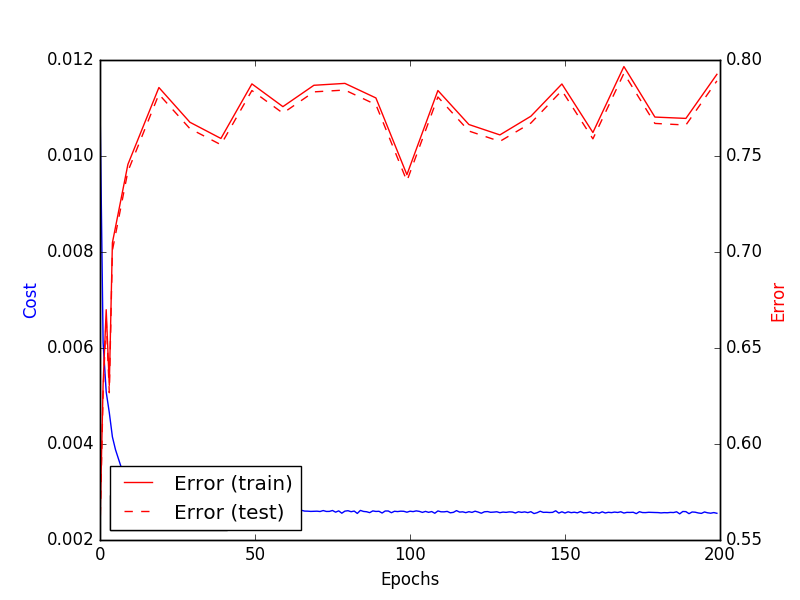
\includegraphics[scale=0.6]{alphaUnsup_SSIM_VALID_SET.png} 
\caption[SSIM validation progress during training of unsupervised alpha network]{SSIM progress over each epoch of unsupervised alpha network on validation dataset.}
\label{fig:alphaUnsupValidSSIM} 
\end{figure}  

\begin{figure}[tb] 
\centering 
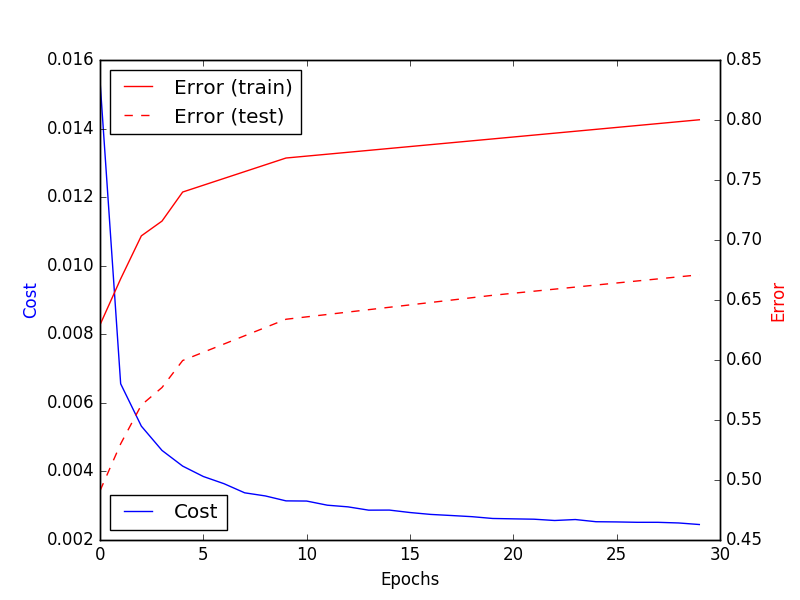
\includegraphics[scale=0.6]{alphaUnsup_SSIM_TEST_SET.png} 
\caption[SSIM testing progress during training of unsupervised alpha network]{SSIM progress over each epoch of unsupervised alpha network on testing dataset.}
\label{fig:alphaUnsupTestSSIM}
\end{figure}  

%The reconstructed images from testing dataset using the unsupervised alpha network is shown %are figure \ref{fig:allReconAlphaUnsup}.

%\begin{figure}[tb] 
%\centering 
%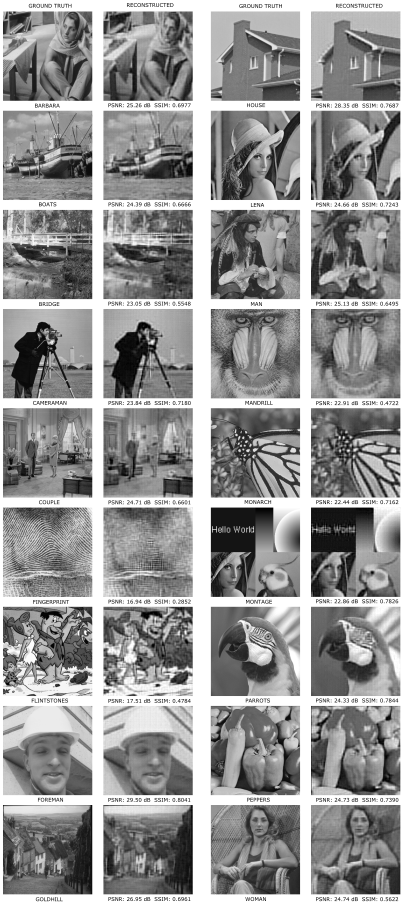
\includegraphics[scale=1]{alphaUnsup_ReconAll.png} 
%\caption[Reconstructed testing images with unsupervised alpha network]{Ground truth, PSNR and %SSIM of reconstructed images from testing dataset using unsupervised alpha network.}
%\label{fig:allReconAlphaUnsup} 
%\end{figure}  

\FloatBarrier

%%%%%%%%%%%%%%%%%%%%%%%%%%%%%%%%%%%BETA%%%%%%%%%%%%%%%%%%%%%%%%%%%%%%%%%%%%%%%%%%%%%%

\section{Beta Network}
Beta network is much deeper compared to alpha network. It was described in section \ref{ch:alphaNet} and in the following we present the results obtained during training.

\subsection{Supervised training}
This approach reconstructs images from compressed measurements. Like alpha networks, we show the results after 200 trainign epochs. Figures \ref{fig:betaSupValidPSNR} and \ref{fig:betaSupTestPSNR} show the progress of PSNR on the validation and testing datasets. Beta network, improves PSNR in 1.1 dB. Figures \ref{fig:betaSupValidSSIM} and \ref{fig:betaSupTestSSIM} show SSIM progress during training for validation and testing datasets. For SSIM, beta network improved it 0.03 with respect alpha network.  
\begin{figure}[tb] 
\centering 
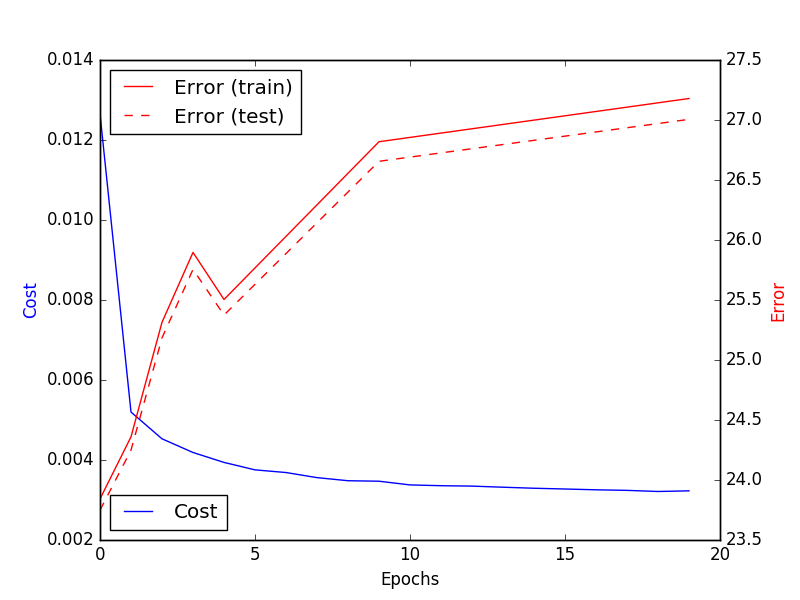
\includegraphics[scale=0.6]{betaSup_PSNR_VALID_SET.png} 
\caption[PSNR validation progress during training of supervised beta network]{PSNR progress over each epoch of supervised beta network on validation dataset.}
\label{fig:betaSupValidPSNR} 
\end{figure}  

\begin{figure}[tb]
\centering 
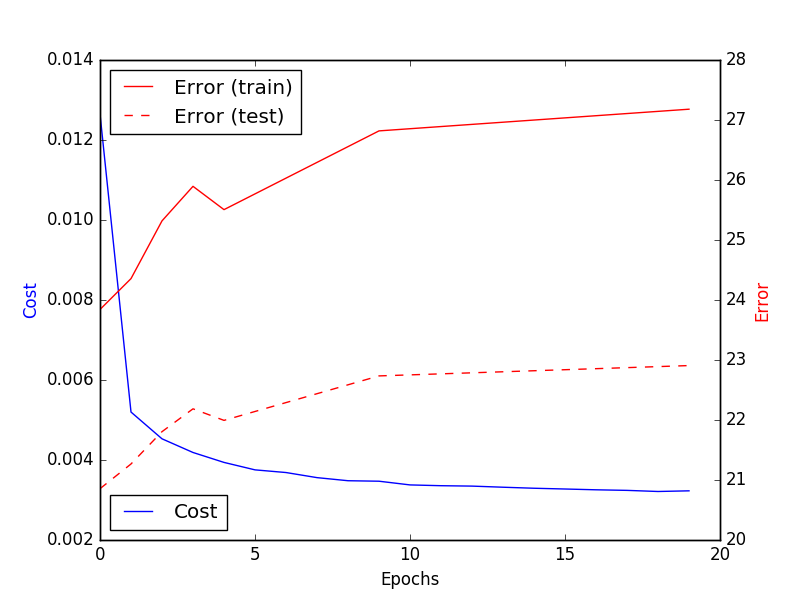
\includegraphics[scale=0.6]{betaSup_PSNR_TEST_SET.png} 
\caption[PSNR testing progress during training of supervised beta network]{PSNR progress over each epoch of supervised beta network on testing dataset.}
\label{fig:betaSupTestPSNR} 
\end{figure}  

\begin{figure}[tb] 
\centering 
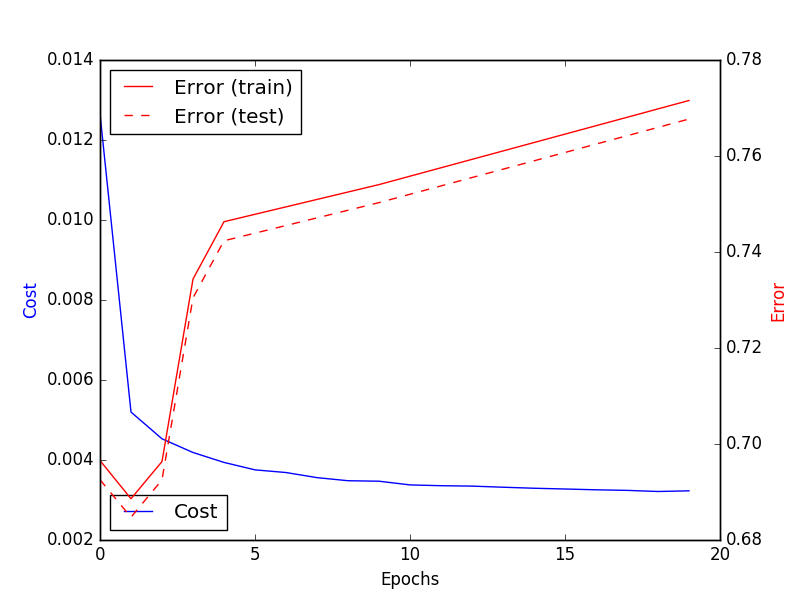
\includegraphics[scale=0.6]{betaSup_SSIM_VALID_SET.png} 
\caption[SSIM validation progress during training of supervised beta network]{SSIM progress over each epoch of supervised beta network on validation dataset.}
\label{fig:betaSupValidSSIM} 
\end{figure}  

\begin{figure}[tb] 
\centering 
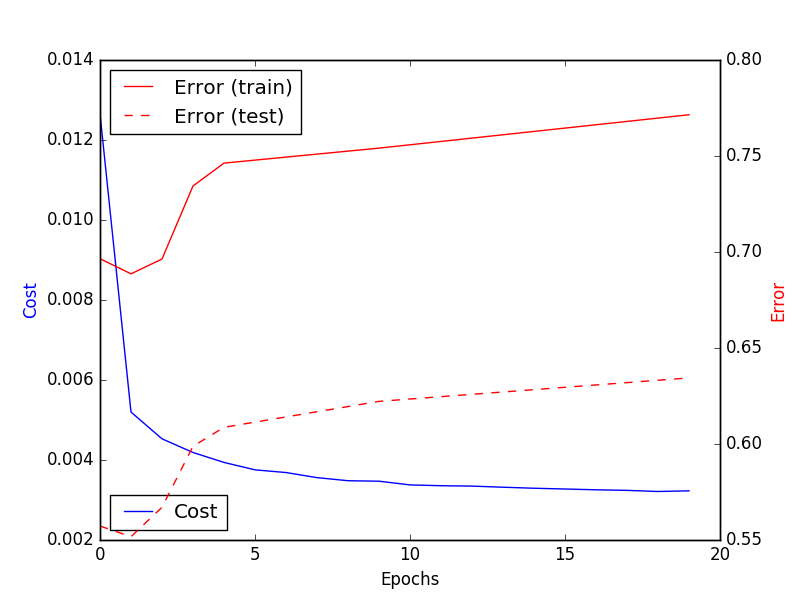
\includegraphics[scale=0.6]{betaSup_SSIM_TEST_SET.png} 
\caption[SSIM testing progress during training of supervised beta network]{SSIM progress over each epoch of supervised beta network on testing dataset.}
\label{fig:betaSupTestSSIM} 
\end{figure}  

\FloatBarrier

\subsection{Unsupervised training}
The traning for unsupervised learning uses the reshaped original images as its input. The compression phase is part of the network architecture and in the following we present the results of the training. Figure \ref{fig:betaUnsupValidPSNR} and \ref{fig:betaUnsupTestPSNR} show the progress in PSNR over each epoch. Compared to the alpha network it improves PSNR by ??????????   

\begin{figure}[tb] 
\centering 
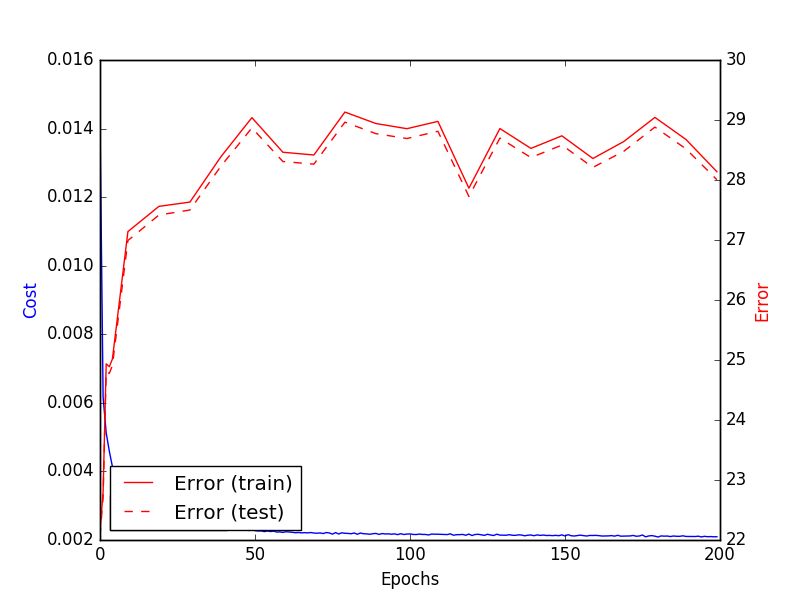
\includegraphics[scale=0.6]{betaUnsup_PSNR_VALID_SET.png} 
\caption[PSNR validation progress during training of unsupervised beta network]{PSNR progress over each epoch of unsupervised beta network on validation dataset.}
\label{fig:betaUnsupValidPSNR} 
\end{figure}  

\begin{figure}[tb] 
\centering 
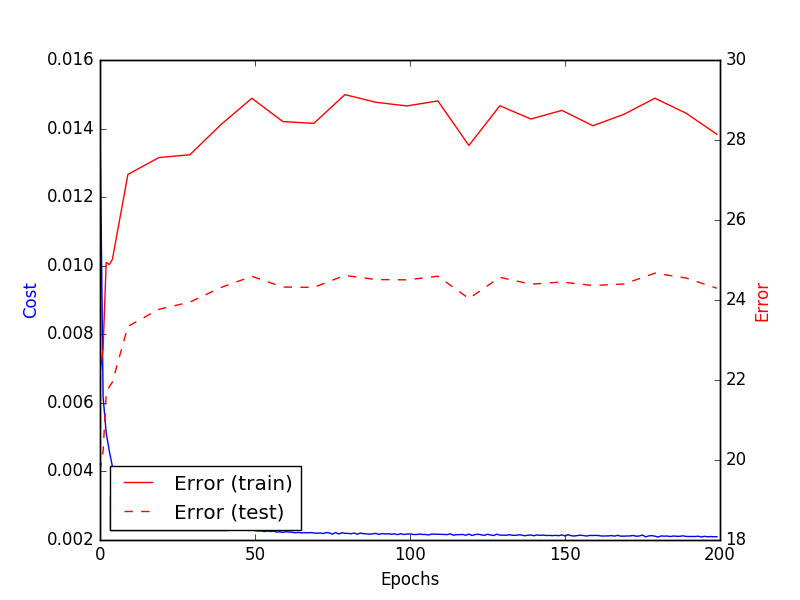
\includegraphics[scale=0.6]{betaUnsup_PSNR_TEST_SET.png} 
\caption[PSNR testing progress during training of unsupervised beta network]{PSNR progress over each epoch of unsupervised beta network on testing dataset.}
\label{fig:betaUnsupTestPSNR} 
\end{figure}  

\begin{figure}[tb] 
\centering 
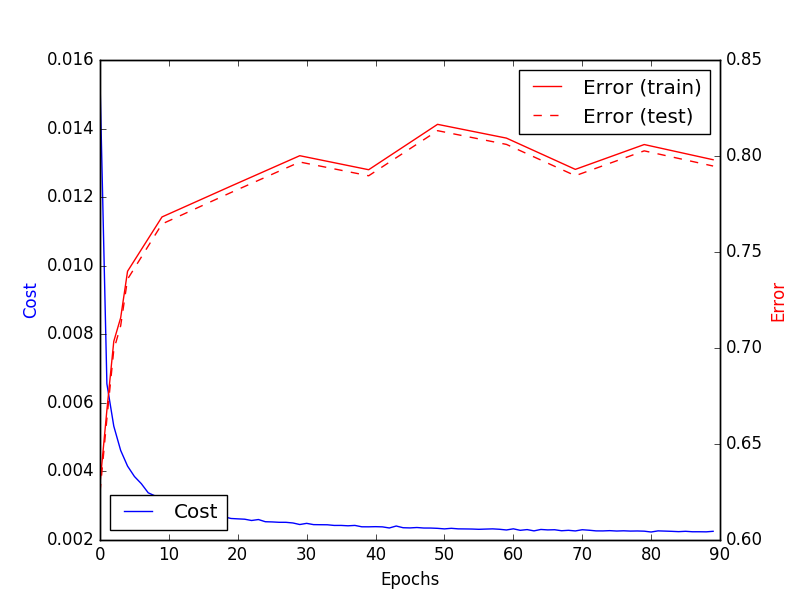
\includegraphics[scale=0.6]{betaUnsup_SSIM_VALID_SET.png} 
\caption[SSIM validation progress during training of unsupervised beta network]{SSIM progress over each epoch of unsupervised beta network on validation dataset.}
\label{fig:betaUnsupValidSSIM} 
\end{figure}  

\begin{figure}[tb] 
\centering 
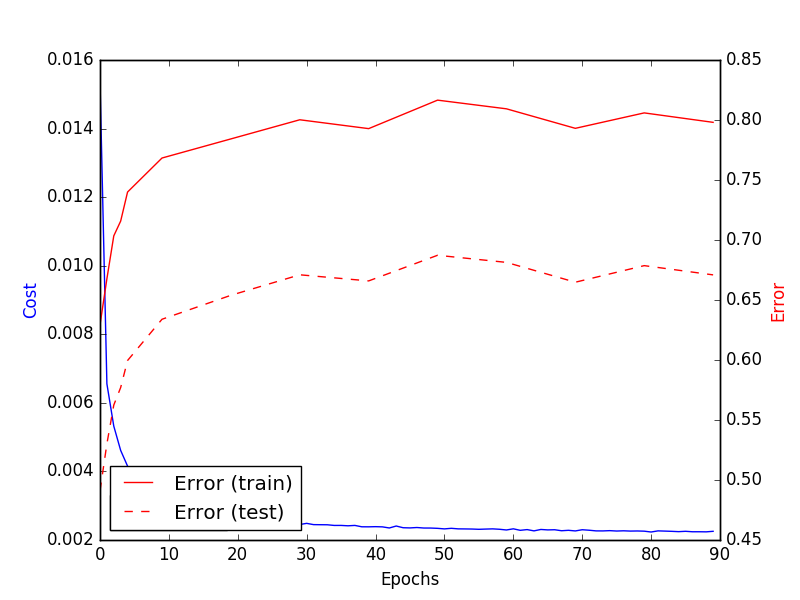
\includegraphics[scale=0.6]{betaUnsup_SSIM_TEST_SET.png} 
\caption[SSIM testing progress during training of unsupervised beta network]{SSIM progress over each epoch of unsupervised beta network on testing dataset.}
\label{fig:betaUnsupTestSSIM} 
\end{figure}  

\FloatBarrier

\section{Summary}
In this section we present a compendium of training and outcome of all proposed architecture networks for recovering the images. Table \ref{tab:summaryPSNR} shows PSNR for each dataset and Table \ref{tab:summarySSIM} does the same for SSIM. Additionaly, we add a colum representing of the denoised image using BM3D\citep{dabov2007image}. Using BM3D does not increase quality considereably but, it helps remove the block representaion. Finally, table \ref{tab:summaryComp} compares our approach against some of the most recognized state-of-the-art algorithms.    
\begin{table}[tb]
\caption[Compendium of PSNR for reconstructing networks]{Comparison in PSNR performance for each proposed network.}
\label{tab:summaryPSNR}
\centering
\begin{tabular}{l*{6}{c}r}
Network              & PSNR TRAINING & PSNR VALIDATION & PSNR TESTING & PSNR TESTING DENOISED\\
\hline
Alpha Supervised   & 26.47 dB & 26.31 dB & 22.37 dB & 22.54 dB\\
Alpha Unsupervised     & 28.19 dB & 28.03 dB & 24.02 dB & 24.24 dB\\
Beta Supervised & 0 dB & 0 dB & 0 dB & 0 dB\\
Beta Unsupervised & 29.14 dB & 28.96 dB & 24.63 dB & 24.77 dB\\
\bottomrule 
\end{tabular}  
\end{table}

\begin{table}[tb]
\caption[Compendium of SSIM for reconstructing networks]{Comparison in SSIM performance for each proposed network.}
\label{tab:summarySSIM}
\centering
\begin{tabular}{l*{6}{c}r}
Network              & SSIM TRAINING & SSIM VALIDATION & SSIM TESTING & PSNR TESTING DENOISED\\
\hline
Alpha Supervised   & 0.7507 & 0.7466 & 0.6062 & 0.6195\\
Alpha Unsupervised     & 0.7925 & 0.7891 & 0.6533 & 0.6715\\
Beta Supervised & 0 & 0 & 0 & 0 \\
Beta Unsupervised & 0.8155 & 0.8124 & 0.6873 & 0.6947\\
\bottomrule 
\end{tabular}  
\end{table}

\begin{table}[tb]
\caption[Timing and qualitz metrics cameranman]{Comparison of reconstructing cameraman with several algorithms with subrate $\frac{1}{16}$.}
\label{tab:summaryComp}
\centering
\begin{tabular}{l*{6}{c}r}
Network              & TIME(sec) & PSNR & SSIM \\
\hline
TVAL3 & 122.12 & 24.15 dB & 0.6896\\
NLR-CS & 0 & 0 & 0 & 0 \\
D-AMP & 0 & 0 & 0 & 0 \\
Alpha Supervised   & 0.7507 & 0.7466 & 0.6062 & 0.6195\\
Alpha Unsupervised     & 0.7925 & 0.7891 & 0.6533 & 0.6715\\
Beta Supervised & 0 & 0 & 0 & 0 \\
Beta Unsupervised & 0.8155 & 0.8124 & 0.6873 & 0.6947\\
\bottomrule 
\end{tabular}  
\end{table}

\FloatBarrier

